% Generated by code/ch11_lindblad_id.py -- do not edit by hand.
\definecolor{qocA}{rgb}{0.00,0.45,0.70}
\definecolor{qocB}{rgb}{0.90,0.60,0.00}
\definecolor{qocC}{rgb}{0.00,0.62,0.45}
\definecolor{qocD}{rgb}{0.80,0.40,0.00}
\definecolor{qocE}{rgb}{0.80,0.60,0.70}
\definecolor{qocF}{rgb}{0.35,0.70,0.90}
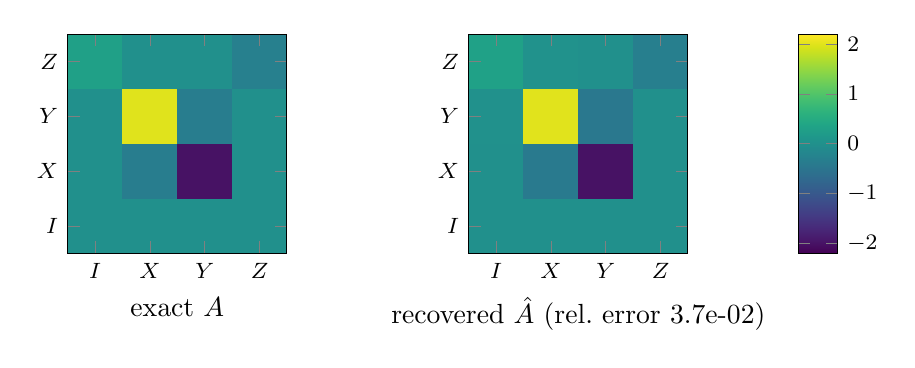
\begin{tikzpicture}[]
\begin{axis}[width=0.36\linewidth, height=0.36\linewidth, xlabel={exact $A$}, ylabel={}, colormap/viridis, enlargelimits=false, axis on top, tick label style={font=\footnotesize}, xtick={0,1,2,3}, ytick={0,1,2,3}, xticklabels={$I$,$X$,$Y$,$Z$}, yticklabels={$I$,$X$,$Y$,$Z$}, point meta min=-2.2, point meta max=2.2]
\addplot[matrix plot*, point meta=explicit, mesh/cols=4] table[meta=z] {
x y z
0 0 0
1 0 0
2 0 0
3 0 0
0 1 0
1 1 -0.35
2 1 -2
3 1 0
0 2 0
1 2 2
2 2 -0.35
3 2 0
0 3 0.3
1 3 0
2 3 0
3 3 -0.3
};
\end{axis}
\begin{scope}[xshift=0.42\linewidth]
\begin{axis}[width=0.36\linewidth, height=0.36\linewidth, xlabel={recovered $\hat A$ (rel.\ error 3.7e-02)}, ylabel={}, colormap/viridis, enlargelimits=false, axis on top, tick label style={font=\footnotesize}, colorbar, xtick={0,1,2,3}, ytick={0,1,2,3}, xticklabels={$I$,$X$,$Y$,$Z$}, yticklabels={$I$,$X$,$Y$,$Z$}, point meta min=-2.2, point meta max=2.2]
\addplot[matrix plot*, point meta=explicit, mesh/cols=4] table[meta=z] {
x y z
0 0 -1.8953e-14
1 0 1.1391e-14
2 0 -3.8038e-16
3 0 1.2707e-14
0 1 -0.0073521
1 1 -0.40361
2 1 -2.0022
3 1 0.0053175
0 2 0.0086909
1 2 2.0033
2 2 -0.43421
3 2 -0.0068988
0 3 0.30491
1 3 0.031091
2 3 -0.0024902
3 3 -0.31483
};
\end{axis}
\end{scope}
\end{tikzpicture}
